\newpage
\section{Expanding LeitnersLearningBox}
\genHeader

\emph{Introduce the problem: four partitions. Integrator doesn't help, what do? Protocol! Explain what went wront, new rule! Run again, show protocol round
two, and look! it runs fine.}

At this point, we now have a working TGG transformation for Dictionary into box with three partitions, and a box with \emph{precisely} three partitions into a
Dictionary. The only forseeable problem here is that\ldots well\ldots exactly three partitions is slightly unrealistic for a proper study box. After all, the
more you need to practice a subject, the more partitions you should have so you are quizzed again and again.

Problem: exactly three partition is kind of unrealistic for a box. After all, the more you want to practice a word, or a set of words, the more partitions you
should have so that you are asked again and again what the answer is. But no matter - our current rule needs at least three to work, right? If a new one is
added, it should still work for those three. Lets confirm by adding a fourth partition to \texttt{source.xmi}. Give it an index of three, set its prev value to
partition2, and set the next value in partition2 to partition3. also set its back to QuestionThree and face to answer dreisave and run TGGMain. it failed (say,
what?!). Even though it was able to find a solution to the first threee, there was no way it could have connected number 4 successfully, resulting in a dangling
edge, which fujaba does not allow.

But why didn't at least the first set of card from partitions 0, 1, 2. Work? Dangling edges - predicts that there will be no way to repair it, so it ends te
whole operation.

While we addressed in index issue in our implemenation code (anzthing above 2 would be assigned as index 2), that only took care of one direction (card to
entry) in the other direction, it simly has no idea what needs to be created /made. 

Lets consider extending the rule so it could handle a fourth card. It would be as simple as including another partition in our rule and connecting it proberly.
But what if we wanted a fith? a sixth?  This obviously won't work -- there will always be an n+1 partition that needs to be resolved.

Instead, let's create a new rule. After all, the protocol is bound to try EVERY possilbilty before continuing. that means, if the first rule fails, it will try
to apply this one, and it will succeed.

\jumpDual{allCards vis}{allCards tex}

\newpage
\hypertarget{allCards vis}{}
\subsection{AllOtherPartitionsRule}
\genHeader

\begin{itemize}

\item[$\blacktriangleright$] Create a new rule \texttt{AllOtherPartitionsRule}, and complete it according to \Cref{fig:ea_AllOtherPartitionsRuleComplete}.


\begin{figure}[htbp]
\begin{center}
  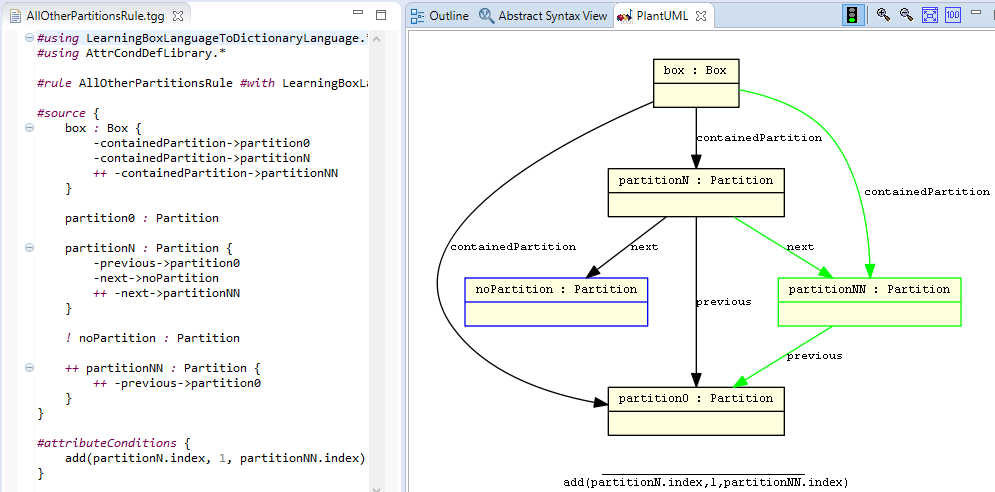
\includegraphics[width=\textwidth]{ea_AllOtherPartitionsRule}
  \caption{The completed \texttt{AllOtherPartitionsRule}}
  \label{fig:ea_AllOtherPartitionsRuleComplete}
\end{center}
\end{figure}

\item[$\blacktriangleright$] As you can see, this rule doesn't assume to know the final \texttt{partition} in the transformation. 
It matches the \texttt{n}th partition as the partition without any next partition, then connects a new \texttt{n+1}th partition to \texttt{n} and \texttt{partition0} (clear as every partitions previous is \texttt{partition0}).
Note that TGG transformations assume that the models are valid, i.e., have the expected structure (in our case meaning that the learning box is correctly ``wired'').\footnote{This should actually be formalised with a set of metamodel constraints that must be checked before a transformation is run, but we've omitted this here to simplify things.}  
Remember that ``blue'' means ``negative''.

\item[$\blacktriangleright$] Generate code for your improved TGG and re-run the transformation. 
It should work now without any error message.
Inspect the protocol to understand what happened.

\item[$\blacktriangleright$] Go ahead and add as many \texttt{partition}s and \texttt{card}s as you like to your model instance.
Your TGG is now also able to handle a \texttt{box} with any number of \texttt{partition}s beautifully.
For five partitions all with cards, the protocol gets quite interesting and is no longer a flat tree.
Try it out! 

\end{itemize}



%%% Local Variables: 
%%% mode: latex
%%% TeX-master: "../src/TGG_mainFile"
%%% End: 


\newpage
\hypertarget{allCards tex}{}
\subsection{AllOtherCardsRule}
\texHeader

\begin{itemize}

\item[$\blacktriangleright$] Right click on the \texttt{rules} folder again and create \texttt{AllOtherCardsRule}. Complete the rule until your file resembles
Fig.~\ref{fig:eclipse_allOtherCardsRule}.

\vspace{0.5cm}

\begin{figure}[htbp]
\begin{center}
  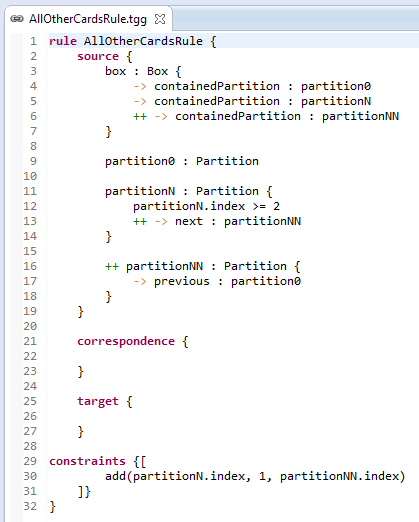
\includegraphics[width=0.7\textwidth]{eclipse_allOtherCardsRule}
  \caption{A complete \texttt{AllOtherCardsRule}}
  \label{fig:eclipse_allOtherCardsRule}
\end{center}
\end{figure}

\item[$\blacktriangleright$] You'll notice that \texttt{box} and \texttt{partition0} have been established as `black' objects -- this rule may only be evaluated
when these objects are already known (and simply need to be adjusted), so we can use their values from the context of the transformation.

\vspace{0.5cm}

\item[$\blacktriangleright$] A second partition, \texttt{partitionN}, has also been established from the context. It represents the \texttt{n}th or last
partition in a \texttt{box} (with an index of 2 or higher), whose \texttt{next} reference will be updated in order to provide an access
link to the newest element, \texttt{partitionNN}.

\newpage

\item[$\blacktriangleright$] Given that the \texttt{add(a,b,c)} syntax is \texttt{a+b=c}, the sole constraint of this rule sets the \texttt{index} of the
\texttt{n+1}th partition so that the \texttt{partition}s are still listed in order.

\vspace{0.5cm}

\item[$\blacktriangleright$] That's it! Save and build your package explorer, then run the TGG again with the `extra' \texttt{partition} to confirm it worked!
You are now free to add as many \texttt{partition}s and \texttt{card}s to \texttt{source.xmi} -- the transformation is now able to elegantly handle them all.

\vspace{0.5cm}

\item[$\blacktriangleright$] Be sure to check out how this rule is implemented in eMoflon's visual specification with Fig.~\ref{fig:ea_allOtherCardsRule} from
the previous section.

\end{itemize}


\newpage
\section{The Protocol Explained}
\genHeader

% files are saved and built/refereshed in the Eclipse workspace.

Now that everything is working correctly, let's return to one of the generated protocol files and quickly review what happens in greater detail. Though it looks
scary, this file can prove to be useful if the integrator was ever to fail again, or if you simply wanted to know more detail about what happened during the
transformation process.

\ldots

